%% This document gives an example on how to use the ntnumasterthesis
%% LaTeX document class.

%% Use short name MACS, MIS, CIMET, MTDMT, MIXD or MIS  
%% Language english or norsk
%% b5paper with oneside or twoside, you can set A4 if you want but you submit in b5

%% If you want print with the heading material on a4 paper you can use this format
%% \documentclass[MACS,english,a4paper,oneside,12pt]{ntnuthesis/ntnuthesis}

%% with the change to using DAIM we have a new option. include DAIM after english below removes the front page material so that you can then submit in the DAIM system. If you are wanting the front material remove DAIM and make sure you fill in the DaimData.tex file.
\documentclass[MACS,english]{ntnuthesis/ntnuthesis}

\usepackage[T1]{fontenc}
\usepackage[utf8]{inputenc}     % For utf8 encoded .tex files allows norwegian characters in the files. This can be dangerous if you change to a differnt editor.
%\usepackage[pdftex]{graphicx, hyperref}   % For cross references in pdf
\usepackage{graphicx}
\usepackage{hyperref}   % For cross references in pdf
\graphicspath{ {figures/} }


\usepackage{color}              % For colouring text 
\hypersetup{colorlinks=true,     
		linkcolor=blue,          % color of internal links (change box color with linkbordercolor)
    citecolor=blue,        % color of links to bibliography
    filecolor=blue,      % color of file links
    urlcolor=blue           % color of external links
		}
\usepackage{csvsimple}  % for simple table reading and display
\usepackage{url}
\usepackage{booktabs}
\usepackage{gnuplottex} %miktex option if using miktex on windows
\usepackage{rotating}


\definecolor{darkgreen}{rgb}{0,0.5,0}
\definecolor{darkred}{rgb}{0.5,0.0,0}

\lstset{        basicstyle=\ttfamily,
                keywordstyle=\color{blue}\ttfamily,
                stringstyle=\color{darkred}\ttfamily,
                commentstyle=\color{darkgreen}\ttfamily,
}


%Typesetting of C++ but not always stable in titles etc...
\newcommand{\CPP}[0]{{C\nolinebreak[4]\hspace{-.1em}\raisebox{.1ex}{\small\bf +\hspace{-.1em}+\ }}}

%\usepackage[table]{xcolor}% http://ctan.org/pkg/xcolor
%\usepackage[nomessages]{fp}
%\newlength{\maxbarlen}


\newcommand\databar[3][gray!20]{%
  \FPeval\result{round(#3/#2:4)}%
  \rlap{\textcolor{#1}{\hspace*{\dimexpr-\tabcolsep+.5\arrayrulewidth}%
        \rule[-.05\ht\strutbox]{\result\maxbarlen}{.95\ht\strutbox}}}%
  \makebox[\dimexpr\maxbarlen-2\tabcolsep+\arrayrulewidth][r]{#3}}



\newcommand{\com}[1]{{\color{red}#1}} % supervisor comment
%\renewcommand{\com}[1]{} %remove starting % to remove supervisor comments
% This will appear in text \com{Lecuters comment} and be visible unless you uncomment
% the renewcommand line.

\newcommand{\todo}[1]{{\color{green}#1}} % items to do
%\renewcommand{\todo}[1]{} %remove starting % to remove items to do

\newcommand{\n}[1]{{\color{blue}#1}} % other comment
%\renewcommand{\n}[1]{} %remove starting % to remove notes

\newcommand{\dn}[1]{} % add the d to a note to say that you have finished with it.





% Set to true ONLY if using Harvard citation style
\newboolean{HarvardCitations}
\setboolean{HarvardCitations}{false} % false for computer science, true for interaction design and harvard style


\ifthenelse{\boolean{HarvardCitations}}{%
	\usepackage{natbib} % for Harvard names as citations.
}{%
	\usepackage[numbers]{natbib} % for Vancover numbers in bibliography
}

\newcommand{\q}[1]{\leavevmode\marginpar{\small\em #1}}
\renewcommand{\q}[1]{}


\begin{document}

% for students submitting in the DAIM system this information will not be used.
% their is an option for DAIM submission which removes this information and checks it is B5.
% Removing the DAIM option on the document type will use this material.

\setthesistitle{Using distributed ledgers for identification in the physical world}
\setthesisshorttitle{Using distributed ledgers for identification in the physical world} % a short version for the page headers if your normal title is too long to fit
\setthesisauthor{J{\o}rgen Ellingsen}
\setthesissupervisor{Assoc. Prof. Mariusz Nowostawski}
\setthesissupervisorA{Prof. Slobodan Petrovic}  % if you have a second supervisor add it like this
%\setthesissupervisorB{Prof. Smart Guy}  % if you have a second supervisor add it like this


\nmtkeywords{Thesis, Latex, Template, IMT}
%\nmtdesc{This is the short description of a masters thesis}


\setthesisdate{01-06-2017}
\setthesisyear{2017}



%for CIMET theses you need to see all of these as well

%\setthesiscampus{Gj\o{}vik}
%\setthesisHostInstitution{\NTNU}
%\setthesisHostInstitution{University of Eastern Finland}
%\setthesisHostInstitution{Universit\'e Jean Monnet Saint-Etienne}

%\setthesisjuryA{} %jury names
%\setthesisjuryB{} %jury names
%\setthesisjuryC{} %jury names
%\setthesisjuryD{} %jury names


 % this is the file which contains all the details about your thesis
\makefrontpages % make the frontpages
\input{inc/mastersIntro}

\tableofcontents

\hypersetup{pageanchor=true}

% Comment with a percent to remove figures or tables:
\listoffigures
\listoftables


\chapter{Introduction}
\label{chap:introduction}
In an increasingly digital world, information is valuable for governments and industry alike. Digital industry leaders has built their business on targeted marketing and big data for years, and the public is slowly realizing the scope of their digital identity and the consequences of not owing their own information. The General Data Protection Regulation (GDPR) is taking a large step to ensure that governments and industry is managing personal information correctly, and that the individual is in control of their own information. 

As more and more businesses and governmental entities understand the value of information, we're faced with a new challenge in information security and individual freedom. We're often required to provide proof of identity on physical locations when buying beer or renting a car. This work will explore the feasibility of using distributed ledgers to manage identities by segregating attributes and transfer control of correlation back to the individual. When entering a bar to meet an old friend, the establishment is required to ensure that you're old enough to buy alcohol, but should not automatically be entitled to information like your name and social security number - other attributes often visible on government issued ID cards. 

Several papers on identity management in distributed ledgers has been published in the past, and this research will focus on implementation and management of attribute based identity verification in a physical interaction. 

The challenge around separating attributes are partially solved by previous papers, but for this to be a working solution as a cyber physical identity service, the system must be cheap and fast in order to work in day-to-day activities. In addition, this thesis will suggest what is required both from the device of the Service Provider and from device of the User, and a analysis of the feasibility of using a mobile or a wearable device for this interaction.

Governments and private companies are currently in a position were they control too much information about our private and social life, movement and habits. When you're asked for ID when entering a bar today, you're effectively disclosing social security number, full name, full date of birth, and other attributes about your identity - when the establishment actually only require to know if you are over 18 years old. The same is valid for governmental controls, like driving license - a police officer has pulled you over, without suspicion of any illegal activity, must control that you do indeed have a drivers license, but is not required to know who you are, and what you're doing. 

A distributed ledger is in its nature visible to anyone who care to look, and the attributes of an identity must therefore be cryptographically separated such that only the individual themselves can connect the information and prove that the information is verified by a trusted identity provider. 

The technology of distributed ledgers, and the research done on identity management in blockchain, enables further research were identity providers and identity holders can agree upon attributes that are available only if the identity holder wants to share them - in a system capable of providing secure proof of identity by verified attributes. This can bring the control of information back to the individual, providing privacy and the possibility of revocation of personal information while the identity attributes are still verifiable as genuine from the given identity provider.

The research problem is in this paper to see if a distributed ledger identity management system can be altered or improved such that it is suitable as physical proof of an identity attribute. This will include finding a way to make the current identity management proposals cheap and fast enough to be a viable option for identity management, and analyze what type of devices is needed to be carried around by the individual to physically prove that they have the required attribute(s). Furthermore, both the user and the service provider must be able to trust the system, and would most likely carry a device each, there is a need to determine what controls must be done on each party's device, and how this information is communicated between them.

A solution were an individual could prove one or more attributes to a entity without disclosing their full identity would be beneficial to privacy and anonymity both online and offline. Utilizing the technology for distributed ledgers like Blockchain~\cite{bitcoin2008} or Tangle~\cite{IOTA_Whitepaper}, we can establish such a mechanism by building on the clever use of cryptographic algorithms proposed in previous papers. The blockchain and the Tangle will be discussed later in Section~\ref{related:work}. This will strengthen the control each individual have over their identity and shared information, and will still provide the service providers with the required information. \cite{Azouvi2017} identifies that their solution does not prove zero-knowledge proofs, but relies on lightweight cryptographic primitives. An identity provider will always know the information contained in the attribute, but should not be able to know if and when the attribute was accessed, and for what purpose. Given the example of entrance to a bar, there should be possible to prove that the individual is over a certain age, but the establishment would not require the exact birth date, and the identity provider would not need to know that the individual shared that information.

While Identity Management in distributed ledgers have been explored in the past, it is usually on either the Bitcoin or Etherium blockchain~\cite{Azouvi2017,Augot2017}.  In addition, the previous research have focused on establishing and maintaining an online identity, but does not explore the possibility of physically presenting proof of an online identity.

This thesis will focus on how an identity can be verified in a physical location, and with that there are some new challenges to overcome. This will require almost instant verification, something that likely will require a different ledger than those previously explored for Identity Management. It will also require the User to carry some sort of identity claim, and the Service Provider to have some way of verifying this claim. 

When these challenges are solved, a prototype will be made as a proof of concept. While this prototype can not be planed in detail before a choice of distributed ledger is made, it is likely to be built as a web application such that it can be easily ported to any laptop or smartphone for testing. % includes latex files from the same directory
\chapter{Background}
\label{chap:background}

\section{Definitions and vocabulary}
\label{sec:background_definitions}

\subsection{Identity Owner}
The owner of the digital identity, also known as the user.

\subsection{Identity Provider}
An entity that verifies and signs attributes associated with an identity to provide a certain level of trust in the validity of the information. This could be governmental bodies, banks and other entities that service providers trust.

\subsection{Service Provider}
An entity that provide some sort of service, and in this context is reliant on a knowing some information relating to the identity of the user. An example of this could be a gambling website ensuring their users are over 18 years of age.

\subsection{Claims}
Attributes a user or identity owner presents to a service provider 

\subsection{Decentralized Identifier (DID)}
Open standard from W3C

\subsection{Self-Sovereign Identity (SSI)}
When Self-Sovereign Identity (SSI) is used as a term within this paper, if references a model of identity management that ensures that the user fully owns and controls their own data. This also includes who has access to the attributes and the possibility to add, delete or revoke these attributes at their own discretion. To assure the privacy required by a SSI-model, the attributes must be stored and processed in a secure manner, and segregation of attributes such that anyone other than the owner can connect the different attributes to the identity.

Even though EGIZ Whitepaper on Self-Sovereign Identity~\cite{ssi} is not technically correct on all the blockchain details, they have a good definition on Self-Sovereign Identity that I have used to define SSI in the context of this thesis. This whitepaper also states that a requirement for a self-sovereign identity model is that access to the information is logged. This is a trade-off between privacy and security and is discussed further in INSERT CHAPTER HERE. 
\section{Distributed Ledgers}
\label{sec:background_dlt}
\subsection{Blockchain}
Bitcoin was the first application of a blockchain, and is based on a proof-of-work system to represent a majority decision. The miners collect pending transactions in the network and form potential blocks, illustrated in Figure \ref{fig:blockchain}, and then, hash the contents of this block with an variable nonce to meet a certain criteria~\cite{bitcoin2008}. For Bitcoin this criteria is that the hash must begin with a certain number of zeros, and this number of zeros can be increased or decreased to compensate for variable computational power in the network~\cite{bitcoin2008}. The complexity is varied to maintain around one block per 10 minutes, but the nature of the psudorandomization of hashing algorithms it can be solved in seconds, but it can also take in excess of 20 minutes~\cite{blockchain_info}. As long as the majority of computational power is controlled by nodes not trying to attack the network, the blockchain serves as a ledger of witnessed transactions with proved ownership.

\begin{figure}[ht]
    \centering
    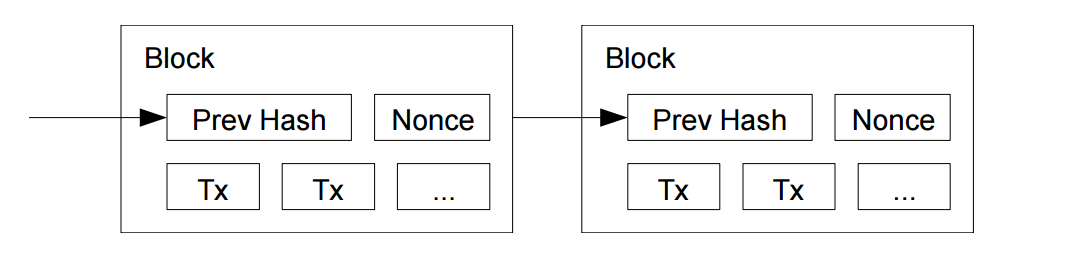
\includegraphics[width=1\textwidth]{blockchain}
    \caption{Visualization of blockchain \cite{bitcoin2008}}
    \label{fig:blockchain}
\end{figure}

The growing success of cryptocurrency, or crypto tokens, the incentive for miners has increased with the price. \cite{VRANKEN20171} estimates the total power consumption to be between 100 and 500 MW, the equivalent of a small nation state, and the inefficiency of the Proof-of-Work (PoW) has made Proof-of-Stake (PoS) look like a strong candidate. In the later years, several PoS currencies has been proposed and launched~\cite{Li2017,nxt_whitepaper,blackcoin_pos} but have yet to achieve large market adoption. The PoS scheme maintain consensus in the network based on the nodes stake, and the consensus is fast and uses negligible resources. PoS implementations sill suffer from some major security concerns, and proposed attacks like~\textit{nothing at stake} and \textit{long-range attacks} is probably holding the adoption back~\cite{Li2017}.

\subsection{Tangle}

The Tangle, here based on the tangle implementation in IOTA~\cite{IOTA_Whitepaper}, provides some very beneficial properties of a Distributed Ledger for Identity Management. The transactions are instant and without traditional fees, and are designed to scale infinitely. The tangle is based on a Directed Acyclic Graph (DAG) rather than a traditional chain of blocks, where each transaction is stored separately in the graph, illustrated in Figure~\ref{fig:tangle}. To make a transaction on the IOTA network, the issuing party must approve two previous transactions, thus strengthening the security of the network. IOTA is still in development, and are still working out some fundamental issues in their implementation. The IOTA foundation recently launched their data market place~\cite{IOTA_Marketplace}, and with this a series of well known industry leaders like Microsoft, Fujitsu, Accenture, and NTNU will participate in the two month beta ending in January/February 2018. IOTA aims to be the backbone of Machine-to-machine and IOT economy.

\begin{figure}[ht]
    \centering
    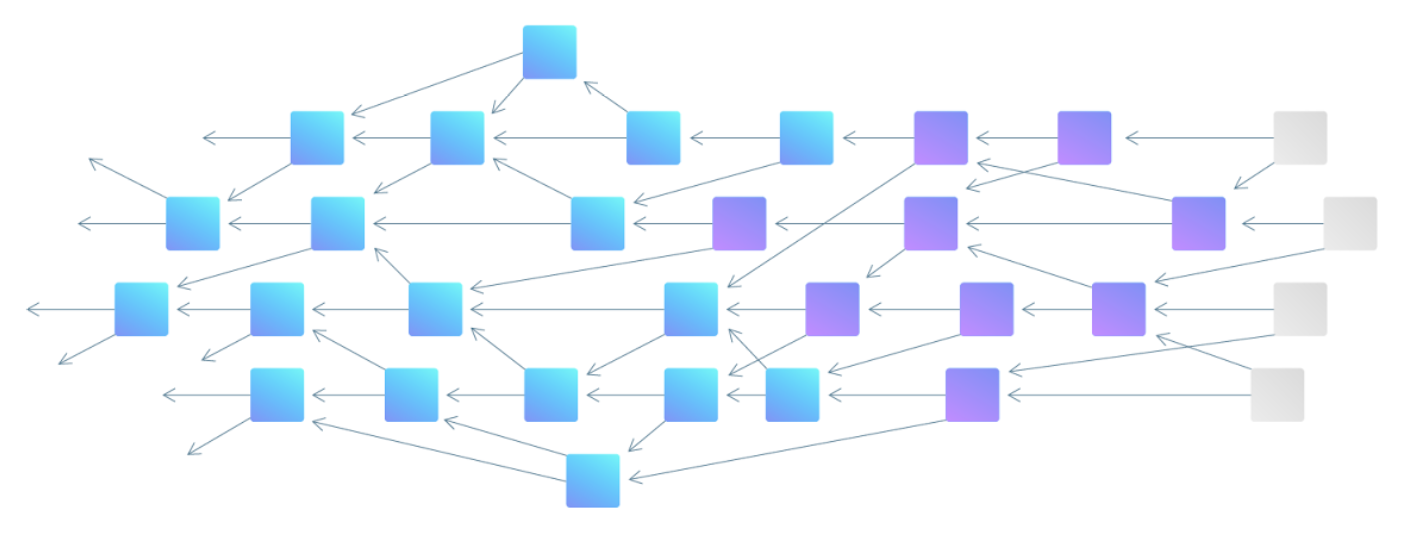
\includegraphics[width=1\textwidth]{tangle}
    \caption{Visualization of the tangle \cite{IOTA_Whitepaper}}
    \label{fig:tangle}
\end{figure}
The web of trust is a public-key authentication system originally built on PGP. A user can build confidence in their identity by having other users sign their public key~\cite{Azouvi2017}. In an identity management system where we distinguish between Users and Service Providers, we can build on this idea. We can look at a scenario where a User has their identity verified and signed by visiting the governmental department issuing passports for their citizens. If the user wants proof that they also have a drivers license, and the issuing body (DMV, Statens Vegvesen, e.g.) trusts that department, they can link a drivers license to that identity based on the verified identity already in the ledger. This opens up for possibilities where the User can visit a small number of Identity Providers and establish a base identity, and then build upon that over the internet.
\chapter{Related Work}
\label{chap:related_work}
Several academic papers propose Identity Management in blockchain applications, and the proposed implementation described in~\cite{Augot2017} provides functionality close to what is required in this system. They propose three types of actors; \textit{Identity Providers} (IP), \textit{Service Providers} (SP) and \textit{Users} (USR), and require three steps in their protocol; \textit{Setup Phase}, \textit{Enrollment Phase}, and \textit{Operational Phase}. In the \textit{Setup Phase}, the \textit{Identity Provider} chooses some set of attributes and makes them publicly available on the Bitcoin ledger. In the \textit{Enrollment Phase}, a \textit{User} brings proof of identity to the \textit{Identity Provider} (Physically or virtually, based on the policy of the \textit{Identity Provider}) that verifies all the attribute values of the claimed identity. This is finalized with a single transaction to the bitcoin ledger, that is considered a \textit{Authentication token}.  In the \textit{Operational Phase} the \textit{User} issues a transaction with the authentication token with outputs to both the \textit{Identity Provider} and back to itself for future transactions. The \textit{Service Provider} issues an Acknowledgement of the identity by sending output from the transaction to the \textit{Identity Provider}. The system is more complicated than described here, with possibilities for revocation and suggestions for storage outside of the blockchain by including the hash of the information in the \textit{OP\_RETURN} instead of the data itself. 

In \cite{Augot2017} the system relies on a Discrete Logarithm Representation (DLREP) proposed in \cite{Brands2000} to efficiently reveal selected parts of an identity to verifiers, while any other information remains hidden. The DLREP can be used to prove boolean functions about the identity, and will satisfy this systems requirement of privacy. 

In~\cite{Azouvi2017} the authors propose several solutions to register identities and attributes in a system built on public ledgers and compare them in terms of privacy, usability and integrity. Two of their solutions satisfy attribute integrity and privacy, and are named \textit{Multi-Casascius} and \textit{Mix-Network}. Both these solutions provide for passive verification, something the authors describes as the possibility to verify the identity only by looking at the public ledger - without the need for additional transactions or information from external sources.
 
\chapter{Technical Solution}
\label{chap:solution}



\begin{itemize}
    \item Hyperledger/Indy/Sovrin https://sovrin.org/wp-content/uploads/Sovrin-Protocol-and-Token-White-Paper.pdf
    \item Blockstack https://blockstack.org/whitepaper.pdf
    \item Multichain https://www.multichain.com/white-paper/
    \item Ethereum http://www.ethdocs.org/en/latest/
    \item uPort https://whitepaper.uport.me/uPort\_whitepaper\_DRAFT20170221.pdf
    \item BlockCerts https://www.blockcerts.org/
    \item Cambridge Blockchain https://www.cambridge-blockchain.com/
    \item Civic https://www.civic.com/
    \item Credits https://credits.com/Content/Docs/TechnicalWhitePaperCREDITSEng.pdf
    \item Evernym  https://www.evernym.com/
\end{itemize}

The DLREP function is a collection of functions proposed by \cite{Brands2000}, and used by \cite{Augot2017}. The instance generator outputs a tuple \[(q, g_1, g_2,...,g_l)\]

\section{Hyperledger Infrastructure}

\section{Indy Framework}

\section{Sovrin Protocol and Token}
The Sovrin Foundation have set out on a mission to standardize and create an infrastructure for Self-Sovereign identities, using blockchain as storage for Distributed Identities such that anyone can issue or verify it~\cite{sovrin}. The Sovrin blockchain has been designed only for identity, and is taking steps to move the digital trust away from centralized CAs to a web of trust model. The Soverin SSI model is not dependent on any particular distributed ledger, but can work with any blockchain that meets the fundamental principles. Sovrin has implemented their identity system in a specific instantiation of Hyperledger's Indy project

%\include{inc/packages} 
%\include{inc/structure} 
%\include{inc/implementation}
%\include{inc/discussion}
%\include{inc/conclusion}

\ifthenelse{\boolean{HarvardCitations}}{%
	\bibliographystyle{agsm} % used for Harvard style references. Names - Humanities & Interaction Design
}{%
	\bibliographystyle{ntnuthesis/ntnuthesis} %used for Vancover style references. Numbers - Computer Science & Physics
}

\bibliography{bibliography}

\appendix
%\include{inc/rawdata}
%\include{inc/timetable}

\end{document}
